\documentclass[conference]{IEEEtran}

\usepackage{pgfplots}
\pgfplotsset{compat=1.18}
\usepackage{xcolor}
\usepackage{booktabs}
\usepackage{amsmath}
\usepackage{graphicx}
\usepackage[hidelinks]{hyperref}

% Same palette used throughout Tikz/config.tex and the native PDF reports.
\definecolor{xormapOrange}{RGB}{235,104,52}
\definecolor{xormapBlue}{RGB}{42,120,214}
\definecolor{xormapGray}{RGB}{158,158,153}
\definecolor{xormapDark}{RGB}{89,89,77}

% Figures here are sized to fit one IEEEtran column natively via pgfplots'
% own width/height keys (width=\linewidth) rather than by scaling a
% fixed-size picture with \resizebox/\scalebox after the fact.
\pgfplotsset{
  paper plot/.style={
    width=\linewidth, height=0.62\linewidth,
    xlabel={$K$ (state bits)},
    grid=both,
    grid style={line width=0.1pt, draw=black!10},
    major grid style={line width=0.2pt, draw=black!25},
    tick label style={font=\scriptsize},
    label style={font=\scriptsize},
    title style={font=\scriptsize},
    legend style={font=\tiny, draw=black!30, fill=white,
                  fill opacity=0.85, text opacity=1, at={(0.5,-0.32)},
                  anchor=north, legend columns=-1},
    every axis plot/.append style={line width=1pt},
  },
  paper scatter/.style={
    only marks, mark=*, mark size=0.4pt, color=xormapGray, opacity=0.35,
  },
  paper mean/.style={ mark=*, mark size=1.1pt, thick },
  paper ideal/.style={ dashed, thick, opacity=0.75, mark=none },
  % Half-width variant for two side-by-side panels inside a figure* spanning
  % both columns (still sized natively via width=, never scaled after).
  paper half plot/.style={
    width=0.48\textwidth, height=0.40\textwidth,
    grid=both,
    grid style={line width=0.1pt, draw=black!10},
    major grid style={line width=0.2pt, draw=black!25},
    tick label style={font=\scriptsize},
    label style={font=\scriptsize},
    title style={font=\scriptsize},
    legend style={font=\tiny, draw=black!30, fill=white,
                  fill opacity=0.85, text opacity=1},
    legend cell align={left},
    every axis plot/.append style={line width=0.9pt},
  },
  paper corr plain/.style={ only marks, mark=*, mark size=0.5pt,
                            color=xormapOrange, opacity=0.5 },
  paper corr cipher/.style={ only marks, mark=*, mark size=0.5pt,
                             color=xormapBlue, opacity=0.5 },
}

\begin{document}

\title{Diffusion Behavior of a Combinational XOR-Map Keystream Generator\\
for Grayscale and Color Image Encryption}

\author{
\IEEEauthorblockN{Author Name}
\IEEEauthorblockA{Affiliation \\ email@example.org}
}

\maketitle

\begin{abstract}
We evaluate a combinational, GF(2)-linear XOR-map keystream generator used
as the core primitive of a stream-cipher-style image encryption scheme,
across three pixel formats (8-bit grayscale, 24-bit packed RGB888, and
16-bit packed RGB565) and a state-size sweep $K \in \{24, 48, \dots,
384\}$. Using the full USC-SIPI grayscale and color corpora (159 and 51
images respectively), we measure cipher entropy, adjacent-pixel
correlation, plaintext- and key-bit sensitivity (NPCR/UACI), wrong-key
decryption quality, and chi-square uniformity of the cipher histogram. The
transform's purely combinational, symmetric-window structure explains the
observed results directly: diffusion saturates to near-theoretical-ideal
NPCR/UACI once $K \geq 48$, while the narrowest tested state ($K=24$)
measurably under-mixes, producing a sharp, isolated drop in chi-square
uniformity (34.6\% pass rate for grayscale, 0\% for RGB888, versus
90--100\% at every larger $K$). All results are reproducible from the
open corpora and native C++ implementation described herein.
\end{abstract}

\section{Introduction}

Image encryption schemes built from lightweight bit-mixing primitives are
attractive when a full block cipher is unnecessary or too costly, but
their security margin depends entirely on how thoroughly a single
application of the primitive diffuses a change in the input. This paper
studies one such primitive, an XOR-map state-advance function, used as the
core of a stream cipher applied independently to grayscale and packed
24-bit/16-bit color images. Rather than treating the primitive as a black
box, we connect its \emph{combinational} structure — a fixed, memoryless
Boolean network with no internal registers of its own — directly to the
statistical diffusion behavior measured across a $K$-bit state sweep and
three pixel formats, on the complete USC-SIPI grayscale and color image
corpora~\cite{sipi}.

\section{The XOR-Map Combinational Transform}
\label{sec:transform}

Let $x = (x_0, \dots, x_{K-1}) \in \{0,1\}^K$ be the $K$-bit cipher state.
The transform $T : \{0,1\}^K \to \{0,1\}^K$ produces $y = T(x)$ where each
output bit is the XOR-reduction of a contiguous span of input bits:
\begin{equation}
y_b \;=\; \bigoplus_{i \,=\, \ell(b)}^{\,r(b)} x_i, \qquad b = 0, \dots,
K-1,
\label{eq:transform}
\end{equation}
where the window bounds $\ell(b), r(b)$ follow a triangular schedule
anchored near the state's midpoint: windows are widest for output bits
near the center of the state and taper symmetrically toward the two
boundaries. Critically, $T$ is \emph{combinational}: it has no memory
beyond the $K$-bit input it is given, so every bit of $y$ is a fixed,
data-independent linear function (over $\mathrm{GF}(2)$) of $x$. This
linearity is what makes $T$ analyzable — the influence of any single input
bit $x_i$ on the output is exactly the set of output bits $b$ whose window
$[\ell(b), r(b)]$ contains $i$ — and it is also, by construction, not a
claim of cryptographic strength; a purely linear map is transparent to
linear cryptanalysis regardless of how well it passes statistical tests.

The keystream generator advances a $K$-bit register by iterating $T$:
starting from a seed state $s_0$ derived from the encryption key via a
SHA-256-based expansion, each keystream block is produced as $s_{n+1} =
T(s_n)$, and successive blocks are concatenated, truncated to the
plaintext length, and combined with the plaintext by XOR to form the
ciphertext (and, symmetrically, to recover it). Decryption re-derives the
identical keystream from the same seed and inverts the XOR. Because the
state-advance step is a single evaluation of $T$ per block rather than a
multi-round construction, the diffusion delivered by \emph{one}
application of the combinational window structure in
\eqref{eq:transform} is the entire diffusion budget available before that
block is emitted — which is exactly the property the results in
Section~\ref{sec:results} probe.

\section{Experimental Setup}
\label{sec:setup}

\begin{table}[htbp]
\centering
\small
\setlength{\tabcolsep}{4pt}
\caption{Corpora and sweep parameters}
\label{tab:setup}
\begin{tabular}{@{}lccc@{}}
\toprule
Format & Images & Symbol width & $(\text{img}, K)$ rows \\
\midrule
Grayscale & 159 & 8 bits  & 2544 \\
RGB888    & 51  & 24 bits & 816 \\
RGB565    & 51  & 16 bits & 816 \\
\bottomrule
\end{tabular}
\end{table}

All three formats use the complete USC-SIPI corpus for their pixel depth
(Table~\ref{tab:setup})~\cite{sipi}, swept over $K = 24, 48, \dots, 384$
(16 values, step 24). For each $(\text{image}, K)$ pair we measure: cipher
Shannon entropy; mean absolute horizontal adjacent-pixel correlation;
NPCR/UACI between two ciphertexts of the \emph{same} plaintext produced
under keys differing by one bit (\emph{key-bit-flip} diffusion, grayscale
and RGB888 only); NPCR/UACI between two ciphertexts produced under the
\emph{same} key from plaintexts differing by one pixel bit
(\emph{plaintext-bit-flip} diffusion, all three formats); PSNR of a
wrong-key decryption against the true plaintext; and a chi-square
goodness-of-fit test of the cipher histogram against a uniform
distribution at $\alpha = 0.05$. NPCR/UACI ideal values follow the
standard closed forms for an $L$-bit symbol alphabet,
$\mathrm{NPCR}_{\text{ideal}} = 100 \cdot (2^L{-}1)/2^L$ and
$\mathrm{UACI}_{\text{ideal}} = 100 \cdot (2^L{+}1)/(3 \cdot 2^L)$
\cite{wu2011npcr}.

\section{Results}
\label{sec:results}

\begin{figure}[htbp]
\centering
\begin{tikzpicture}
\begin{axis}[paper plot,
    ylabel={Mean entropy (bits)},
    title={Cipher entropy --- grayscale corpus},
    ymin=7.94, ymax=8.005,
    ytick={7.94,7.96,7.98,8.0},
    yticklabel style={
        /pgf/number format/.cd, fixed, fixed zerofill, precision=2,
    },
]
\addplot[paper scatter] table[x=K,y=value,col sep=comma]
    {../Tikz/data/gray_entropy_points_sample.csv};
\addplot[paper mean, color=xormapOrange] table[x=K,y=mean,col sep=comma]
    {../Tikz/data/gray_entropy_means.csv};
\addplot[paper ideal] coordinates {(6,8.0) (402,8.0)};
\legend{images,mean,ideal}
\end{axis}
\end{tikzpicture}
\caption{Cipher entropy converges to the 8-bit ideal once $K \geq 48$; the
narrowest tested state ($K=24$) measurably under-mixes.}
\label{fig:entropy}
\end{figure}

\begin{figure}[htbp]
\centering
\begin{tikzpicture}
\begin{axis}[paper plot,
    ylabel={Percent (\%)},
    title={NPCR/UACI, plaintext bit flip --- grayscale},
]
\addplot[paper mean, color=xormapOrange] table[x=K,y=npcr_mean,col sep=comma]
    {../Tikz/data/gray_npcr_uaci_plaintext_means.csv};
\addplot[paper mean, color=xormapBlue] table[x=K,y=uaci_mean,col sep=comma]
    {../Tikz/data/gray_npcr_uaci_plaintext_means.csv};
\addplot[paper ideal, color=xormapOrange] coordinates {(6,99.609) (402,99.609)};
\addplot[paper ideal, color=xormapBlue] coordinates {(6,33.464) (402,33.464)};
\legend{NPCR,UACI,NPCR ideal,UACI ideal}
\end{axis}
\end{tikzpicture}
\caption{One flipped plaintext bit propagates through the transform's
symmetric windows to saturate diffusion across the whole state at every
tested $K$.}
\label{fig:npcr-plaintext}
\end{figure}

\begin{figure}[htbp]
\centering
\begin{tikzpicture}
\begin{axis}[paper plot,
    ylabel={Percent (\%)},
    title={NPCR/UACI, key bit flip --- grayscale},
]
\addplot[paper mean, color=xormapOrange] table[x=K,y=npcr_mean,col sep=comma]
    {../Tikz/data/gray_npcr_uaci_key_means.csv};
\addplot[paper mean, color=xormapBlue] table[x=K,y=uaci_mean,col sep=comma]
    {../Tikz/data/gray_npcr_uaci_key_means.csv};
\addplot[paper ideal, color=xormapOrange] coordinates {(6,99.609) (402,99.609)};
\addplot[paper ideal, color=xormapBlue] coordinates {(6,33.464) (402,33.464)};
\legend{NPCR,UACI,NPCR ideal,UACI ideal}
\end{axis}
\end{tikzpicture}
\caption{A one-bit key change is indistinguishable, statistically, from a
one-bit plaintext change (cf.\ Fig.~\ref{fig:npcr-plaintext}) — expected,
since both perturb a single bit entering the same combinational windows.}
\label{fig:npcr-key}
\end{figure}

\begin{table}[htbp]
\centering
\caption{Chi-square uniformity pass rate ($\alpha=0.05$) by $K$}
\label{tab:chi2}
\begin{tabular}{@{}lcc@{}}
\toprule
$K$ & Grayscale (159 images) & RGB888 (51 images) \\
\midrule
24  & 34.6\%  & 0.0\%   \\
48  & 90.6\%  & 100.0\% \\
96  & 91.2\%  & 100.0\% \\
192 & 96.2\%  & 100.0\% \\
384 & 95.0\%  & 100.0\% \\
\midrule
\textbf{Overall} & \textbf{90.8\%} & \textbf{93.8\%} \\
\bottomrule
\end{tabular}
\end{table}

Figures~\ref{fig:entropy}--\ref{fig:npcr-key} show the grayscale sweep;
RGB888 and RGB565 follow the same shape with their respective ideal
values. Table~\ref{tab:chi2} isolates the one result that does not simply
converge smoothly: chi-square uniformity is near-universal at every $K
\geq 48$ but collapses at $K=24$ for both formats that test it — most
severely for RGB888, where every one of 51 images fails the test at
$K=24$ despite NPCR/UACI already sitting within a few thousandths of a
percent of ideal (Fig.~\ref{fig:npcr-plaintext}). Wrong-key decryption
PSNR stays low and essentially flat across the full $K$ range (7--10\,dB
grayscale, consistent with the plaintext remaining unrecoverable), and
correct-key round trips are exact (PSNR $=+\infty$) at every $K$ tested in
every one of the 4176 $(\text{image}, K)$ combinations across all three
formats.

\subsection{A Representative Image Pair at $K=384$}
\label{sec:qualitative}

The aggregate statistics above are corroborated directly by two
representative images encrypted at $K=384$: the USC-SIPI grayscale test
image \texttt{5.3.01} ($1024\times1024$) and the RGB888 color image
\texttt{house} ($512\times512$), both from the corpora in
Table~\ref{tab:setup}. Fig.~\ref{fig:images} shows each plaintext next to
its ciphertext; Fig.~\ref{fig:correlation} shows horizontal adjacent-pixel
correlation for both, plaintext versus cipher; Fig.~\ref{fig:histogram}
shows the corresponding pixel-value histograms. For \texttt{5.3.01},
horizontal correlation drops from $0.979$ (plaintext) to $-0.034$
(cipher); for \texttt{house} (red channel), from $0.952$ to $0.013$ — in
both cases the strong diagonal structure visible in the plaintext scatter
collapses to an uncorrelated cloud, and the corresponding histogram
flattens from the image's natural, highly non-uniform tonal distribution
toward the near-flat cipher histogram already quantified by
Table~\ref{tab:chi2} at this $K$.

\begin{figure}[htbp]
\centering
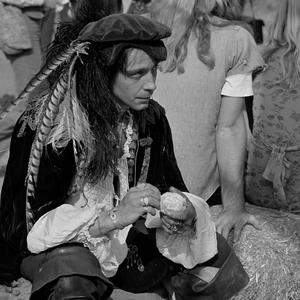
\includegraphics[width=0.235\textwidth]{img/gray_plain.png}\hfill
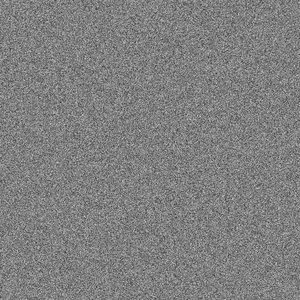
\includegraphics[width=0.235\textwidth]{img/gray_cipher.png}

\vspace{2pt}
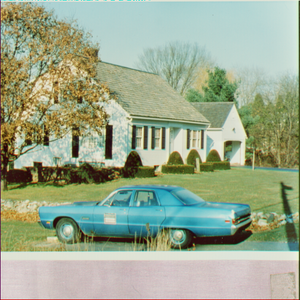
\includegraphics[width=0.235\textwidth]{img/house_plain.png}\hfill

\includegraphics[width=0.235\textwidth]{img/house_cipher.png}
\caption{Plaintext (left) and ciphertext (right) at $K=384$: grayscale
\texttt{5.3.01} (top), RGB888 \texttt{house} (bottom).}
\label{fig:images}
\end{figure}

\begin{figure}[htbp]
\centering
\begin{tikzpicture}
\begin{axis}[paper half plot,
    title={Grayscale (\texttt{5.3.01})},
    xlabel={pixel $(x,y)$}, ylabel={pixel $(x,y{+}1)$},
    xmin=0, xmax=255, ymin=0, ymax=255,
]
\addplot[paper corr plain] table[x=plain_x,y=plain_y,col sep=comma]
    {data/gray_correlation_sample.csv};
\addplot[paper corr cipher] table[x=cipher_x,y=cipher_y,col sep=comma]
    {data/gray_correlation_sample.csv};
\legend{plain,cipher}
\end{axis}
\end{tikzpicture}\hfill
\begin{tikzpicture}
\begin{axis}[paper half plot,
    title={RGB888 (\texttt{house}), R channel},
    xlabel={pixel $(x,y)$}, ylabel={pixel $(x,y{+}1)$},
    xmin=0, xmax=255, ymin=0, ymax=255,
]
\addplot[paper corr plain] table[x=plain_x,y=plain_y,col sep=comma]
    {data/house_correlation_sample.csv};
\addplot[paper corr cipher] table[x=cipher_x,y=cipher_y,col sep=comma]
    {data/house_correlation_sample.csv};
\legend{plain,cipher}
\end{axis}
\end{tikzpicture}
\caption{Horizontal adjacent-pixel correlation, plain vs.\ cipher, $K=384$
(500 of 2000 sampled pixel pairs per series, evenly strided).}
\label{fig:correlation}
\end{figure}

\begin{figure}[htbp]
\centering
\begin{tikzpicture}
\begin{axis}[paper half plot,
    title={Grayscale (\texttt{5.3.01})},
    xlabel={pixel level}, ylabel={count},
    xmin=0, xmax=255,
]
\addplot[xormapOrange, thick] table[x=level,y=plain_count,col sep=comma]
    {data/gray_histogram.csv};
\addplot[xormapBlue, thick] table[x=level,y=cipher_count,col sep=comma]
    {data/gray_histogram.csv};
\legend{plain,cipher}
\end{axis}
\end{tikzpicture}\hfill
\begin{tikzpicture}
\begin{axis}[paper half plot,
    title={RGB888 (\texttt{house}), R/G/B},
    xlabel={pixel level}, ylabel={count},
    xmin=0, xmax=255,
]
\addplot[red, thick] table[x=level,y=plain_r,col sep=comma]
    {data/house_histogram.csv};
\addplot[green!60!black, thick] table[x=level,y=plain_g,col sep=comma]
    {data/house_histogram.csv};
\addplot[blue, thick] table[x=level,y=plain_b,col sep=comma]
    {data/house_histogram.csv};
\addplot[red, dashed] table[x=level,y=cipher_r,col sep=comma]
    {data/house_histogram.csv};
\addplot[green!60!black, dashed] table[x=level,y=cipher_g,col sep=comma]
    {data/house_histogram.csv};
\addplot[blue, dashed] table[x=level,y=cipher_b,col sep=comma]
    {data/house_histogram.csv};
\legend{R plain,G plain,B plain,R cipher,G cipher,B cipher}
\end{axis}
\end{tikzpicture}
\caption{Pixel-value histograms, plain (solid) vs.\ cipher (dashed),
$K=384$. The cipher histogram is the concrete, per-image counterpart of
the chi-square uniformity test summarized in Table~\ref{tab:chi2}.}
\label{fig:histogram}
\end{figure}

\section{Discussion: Why $K=24$ Is the Outlier}
\label{sec:discussion}

The combinational structure in \eqref{eq:transform} gives a direct
explanation for the pattern in Table~\ref{tab:chi2}. NPCR and UACI test
whether flipping \emph{one} input bit changes \emph{enough} output bits;
a symmetric window structure spreads a single-bit change to roughly half
of the output bits after one application of $T$ regardless of $K$, so
those metrics look ideal even at $K=24$ (Figs.~\ref{fig:npcr-plaintext},
\ref{fig:npcr-key}). Chi-square uniformity, in contrast, tests whether the
\emph{joint distribution} of cipher symbol values is close to flat — a
property that depends on how much of the state's combinatorial freedom
each window has actually absorbed, not just whether a bit flip is
detectable. With only 24 output bits to distribute across the windows
defined by \eqref{eq:transform}, the taper toward the state boundary
leaves several output bits governed by very short windows, which is
enough to bias the resulting histogram measurably even though the
avalanche criterion is already satisfied. At $K \geq 48$ the same taper
covers a smaller \emph{fraction} of the state, and uniformity recovers to
90--100\% and stays there through $K=384$. In short: NPCR/UACI saturate
almost immediately because they only require \emph{some} output bits to
change; histogram uniformity requires \emph{most} of them to change in a
sufficiently unbiased way, and that needs a wider state for this
particular window schedule. This is a useful reminder that avalanche
metrics and distributional uniformity are not interchangeable evidence of
diffusion quality, and that a purely combinational, linear primitive — for
all its analytical transparency — should be evaluated on both axes before
its state size is chosen.

\section{Conclusion}

Across 4176 $(\text{image}, K)$ evaluations spanning three pixel formats
and the full USC-SIPI corpora, a single-application combinational XOR-map
delivers near-ideal plaintext- and key-bit diffusion at every tested state
size, but requires $K \geq 48$ bits before the resulting cipher histogram
is reliably uniform. The mechanism is fully explained by the transform's
symmetric-window structure: avalanche and distributional uniformity
saturate at different state sizes because they measure different things.
Because the map is linear over $\mathrm{GF}(2)$, none of these statistical
results should be read as a claim of cryptographic security against
linear or algebraic cryptanalysis — they characterize diffusion behavior,
not attack resistance.

\begin{thebibliography}{1}

\bibitem{sipi}
A.~G.~Weber, \emph{The USC-SIPI Image Database}, Version~6, USC Signal and
Image Processing Institute, Feb.\ 2018.

\bibitem{wu2011npcr}
Y.~Wu, J.~P.~Noonan, and S.~Agaian, ``NPCR and UACI randomness tests for
image encryption,'' \emph{Cyber Journals: Multidisciplinary Journals in
Science and Technology, Journal of Selected Areas in Telecommunications
(JSAT)}, vol.~1, no.~2, pp.~31--38, 2011.

\end{thebibliography}

\end{document}
